\documentclass[10pt,a4paper]{article}
	
	\usepackage{amsmath,amssymb,amsthm,mathtools,amsfonts}
	\usepackage{breqn}
	\usepackage[utf8]{inputenc}
	\usepackage[english]{babel}
	\usepackage[T1]{fontenc}
	
	%%%%%%%%%%%%%%%%%%%%%%%%%%%%%%%%%%%%%%%%%%%%%%%%%%%%%%%%%%%%%%%%%%%%%%%%%%%%%% Fonts
	
	\usepackage{fontspec}
	\setmainfont[Numbers=OldStyle]{EB Garamond}
	\newfontfamily\plantinc[Numbers=OldStyle]{Plantin MT Pro Bold Condensed}
	\newfontfamily\plantinsb{Plantin MT Pro Semibold}
	\newfontfamily\garamond[Numbers=OldStyle]{EB Garamond}
	\newfontfamily\plantin[Numbers=OldStyle]{Plantin MT Pro}
	\newfontfamily\wal{Walbaum Com}
	\newfontfamily\klav{Klavika}
	\newfontfamily\klavl{Klavika light}
	\newfontfamily\quotefont[Ligatures=TeX]{Linux Libertine O}
	
	%%%%%%%%%%%%%%%%%%%%%%%%%%%%%%%%%%%%%%%%%%%%%%%%%%%%%%%%%%%%%%%%%%%%%%%%%%%%%% Colors
	
	\usepackage[svgnames]{xcolor}
	
	\definecolor{hgblue}{RGB}{10, 40, 80}
	\definecolor{hgred}{RGB}{140, 10, 10}
	\definecolor{hggrey}{RGB}{215, 215, 210}
	\definecolor{hggreen}{RGB}{145, 205, 205}
	
	%%%%%%%%%%%%%%%%%%%%%%%%%%%%%%%%%%%%%%%%%%%%%%%%%%%%%%%%%%%%%%%%%%%%%%%%%%%%%% Other Graphics
	
	\usepackage{graphicx}
	\graphicspath{{./img/}}
	\usepackage{tikz}
	\usepackage{placeins}
	\usepackage[modulo]{lineno}
	\usepackage{geometry}
	\usepackage{pdfpages}
	
	
	
	\usepackage[pdfborder={0 0 0}]{hyperref} %% Ingen firkant rundt om referencer

	\usepackage{multicol}
	\usepackage{cellspace}
		\setlength\cellspacetoplimit{100pt}
		\setlength\cellspacebottomlimit{100pt}
	\usepackage{tabularx}
		\newcolumntype{b}{>{\hsize=\hsize}>{\centering\arraybackslash}X}
	\usepackage{siunitx}
	\usepackage{cellspace}
		\setlength\cellspacetoplimit{4pt}
		\setlength\cellspacebottomlimit{4pt}
	
	\usepackage{enumitem}% better controls with enumerating
	\usepackage{wrapfig}
		%\setlength{\wrapoverhang}{\marginparwidth}
		%\addtolength{\wrapoverhang}{\marginparsep}
		\setlength{\columnsep}{0pt}
		\setlength{\intextsep}{-10pt}
	\usepackage{caption}
	%\usepackage{dirtytalk}
	%\usepackage{tasks}
	
	

	\setlength{\parskip}{0.5\baselineskip}
	\setlength{\parindent}{0cm}
	
	\setlist[enumerate]{label=\alph*),left=20pt}
	%\setlist[enumerate]{leftmargin=\parindent}
	%\setlist[enumerate]{nosep}
	
	\usepackage{lipsum}
	\usepackage{comment}
	\usepackage{ulem}
	
	%\reversemarginpar
	
	%%%%%%%%%%%%%%%%%%%%%%%%%%%%%%%%%%%%%%%%%%%%%%%%%%%%%%%%%%%%%%%%%%%%%%%%%%%%%% New commands
	
	\newcommand\svar[1]{\newline\textcolor{red}{\textbf{Svar}\\#1}}
	
	\usepackage[h]{esvect}
	\newcommand{\twvect}[2]{\ensuremath{\begin{pmatrix}#1\\#2\end{pmatrix}}}
	
	\newcommand*\quotesize{20}
	\newcommand*{\openquote}
		{\tikz[remember picture,overlay,xshift=-3ex,yshift=-0ex]
			\node (OQ) {\quotefont\fontsize{\quotesize}{\quotesize}\selectfont``};\kern0pt}

	\newcommand*{\closequote}[1]
		{\tikz[remember picture,overlay,xshift=2ex,yshift={#1}]
			\node (CQ) {\quotefont\fontsize{\quotesize}{\quotesize}\selectfont''};}
			
	\newcommand{\qm}[1]{‘‘#1”}
	\newcommand{\iquote}[1]{\begin{quote}\itshape \openquote#1\hfill\closequote{0ex} \end{quote}}

	\newcommand{\source}[1]{\footnote{Source: \href{#1}{#1}}}
	
	\newcommand{\glos}[3]{\dotuline{#1}\marginpar{\scriptsize\textit{#3} #2}}
	
	\newcommand{\subtitle}[1]{\vspace{10pt}\newline\normalsize\plantin #1}
	
	%%%%%%%%%%%%%%%%%%%%%%%%%%%%%%%%%%%%%%%%%%%%%%%%%%%%%%%%%%%%%%%%%%%%%%%%%%%%%% Sections
	
	\usepackage{titlesec}
	\titleformat{\subsection}{\color{hgred}\plantinc\large}{}{}{}
	\titlespacing*{\subsubsection}{0pt}{\baselineskip}{-1\baselineskip} % use \subsubsection*{} for a baselineskip with noindent afterwards
	
	\usepackage{titling}
	\setlength{\droptitle}{-12ex}
	\pretitle{\begin{flushleft}\plantinc\huge\color{hgblue}}
	\posttitle{\par\end{flushleft}}
	\preauthor{\begin{flushleft}\Large}
	\postauthor{\end{flushleft}}
	\predate{\begin{flushleft}}
	\postdate{\end{flushleft}}
	
	\setcounter{secnumdepth}{0}
	
	%%%%%%%%%%%%%%%%%%%%%%%%%%%%%%%%%%%%%%%%%%%%%%%%%%%%%%%%%%%%%%%%%%%%%%%%%%%%%% Header & Footer
	
	\usepackage{bigfoot}
	\DeclareNewFootnote{a}
		\renewcommand{\thefootnotea}{\fnsymbol{footnotea}}
			\newcommand{\footnotes}[1]{\footnotea[2]{#1}} % here you can specify what symbol you want in footnotes
			\newcommand{\footnoted}[1]{\footnotea[3]{#1}} % for a second footnote on a page
			\MakePerPage{footnotes}
	
			%%%%%%%%%%%%%%%%%%%%%%%%%%%%%%%%%%%%%%%%%%%%%%%%%%%%%%%%%%%%%%%%%%%%%%%%%%%%%% Document

\begin{document}
%\pagecolor{FloralWhite}
\title{On Being Crazy}
%\date{\vspace{-3em}} % I tilfældet ingen dato
\date{1907}
\author{W.E.B. Du Bois}

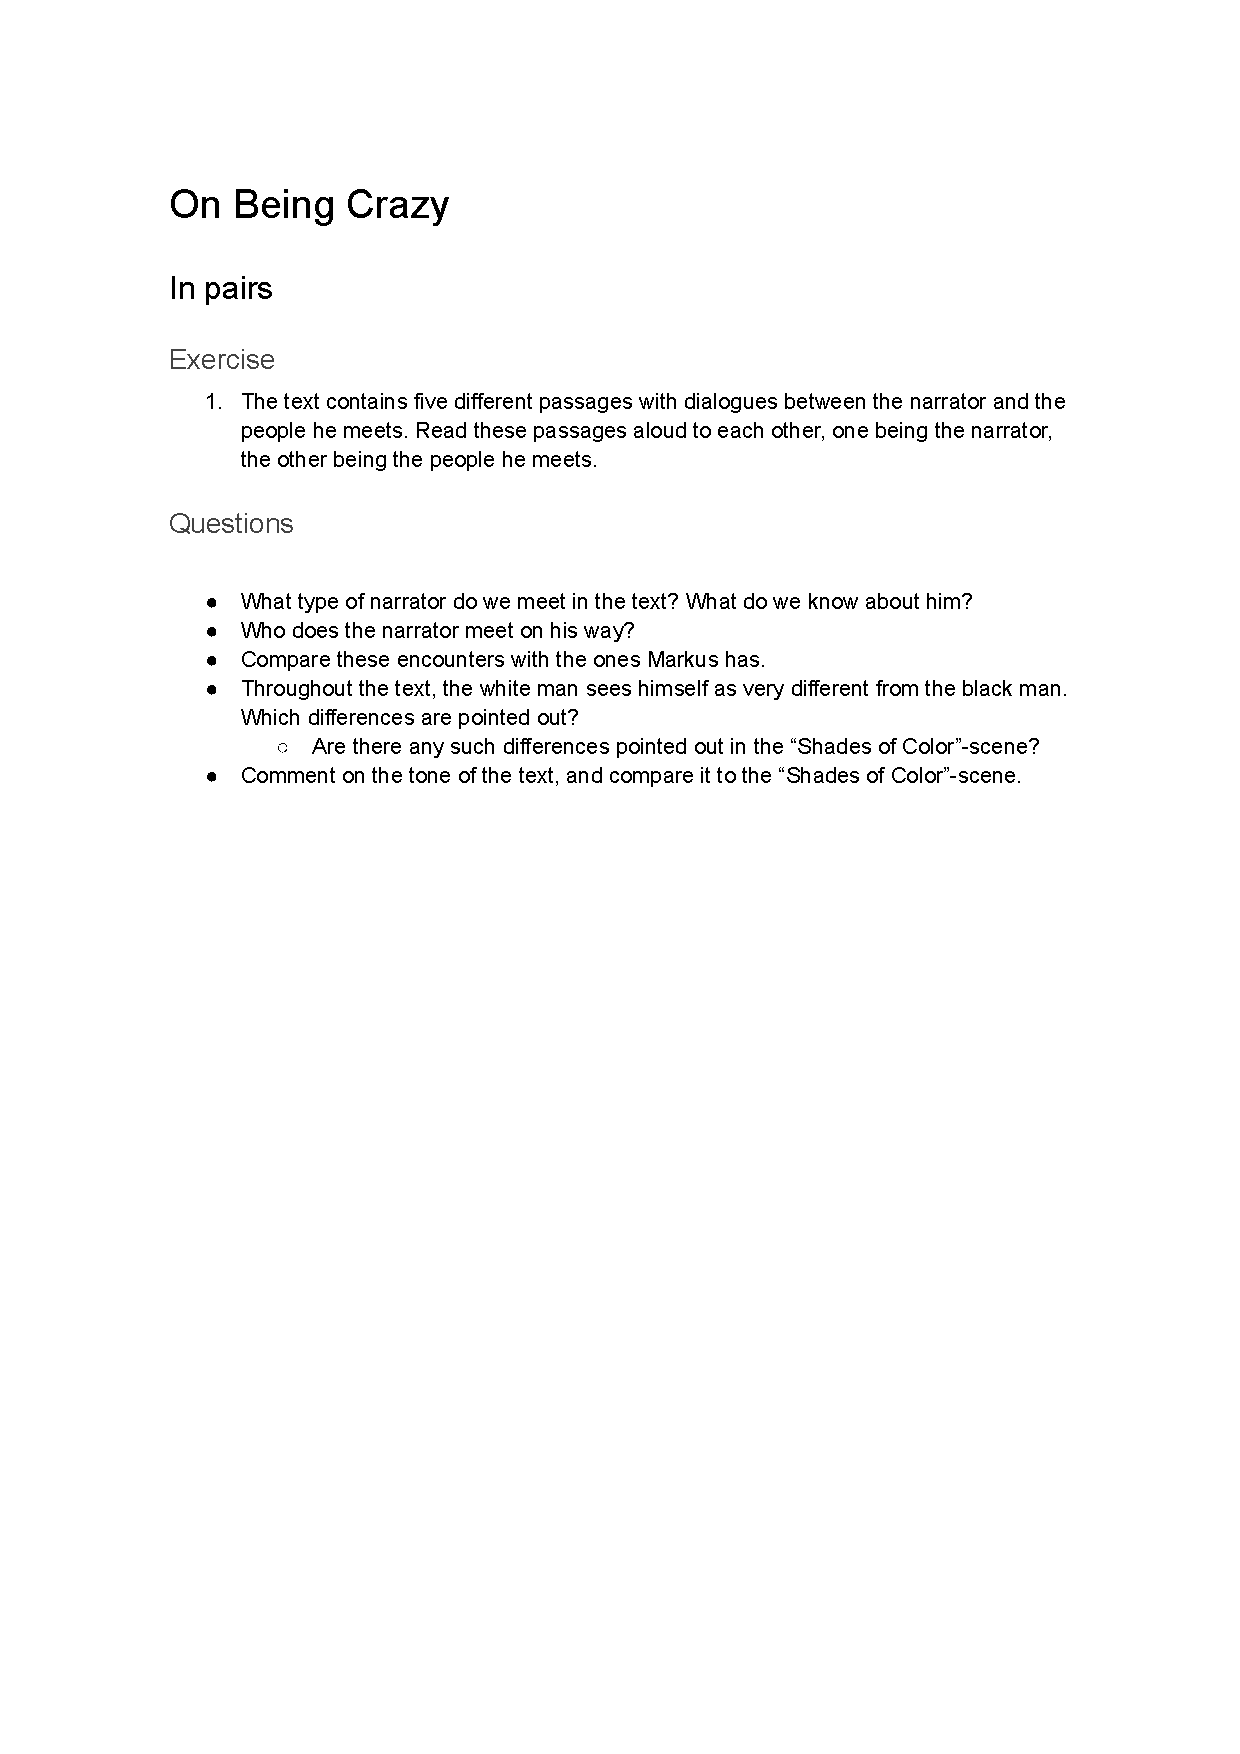
\includepdf{arbejdsark.pdf}

\maketitle
\noindent\linenumbers It was one o’clock and I was hungry. I walked into a restaurant, seated myself, and reached for the bill of fare. My table companion rose.

“Sir,” said he, “do you wish to force your company on those who do not want you?”

No, said I, I wish to eat.

“Are you aware, sir, that this is social equality?”

Nothing of the sort, sir, it is hunger—and I ate.

The day’s work done, I sought the theatre. As I sank into my seat, the lady shrank and squirmed.

I beg pardon, I said.

“Do you enjoy being where you are not wanted?” she asked coldly.

Oh, no, I said.

“Well, you are not wanted here”

I was surprised. I fear you are mistaken, I said, I certainly want the music, and I like to think the music wants me to listen to it.

“Usher,” said the lady, “this is social equality.”

“No madame,” said the usher, “it is the second movement of Beethoven’s Fifth Symphony.”

After the theatre, I sought the hotel where I had sent my baggage. The clerk scowled.

“What do you want?”

Rest, I said.

“This is a white hotel,” he said.

I looked around. Such a color scheme requires a great deal of cleaning, I said, but I don’t know that I object.

“We object,” said he.

Then why, I began, but he interrupted.

“We don’t keep niggers,” he said, “we don’t want social equality.”

Neither do I, I replied gently, I want a bed.

I walked thoughtfully to the train. I’ll take a sleeper through Texas. I’m a little bit dissatisfied with this town.

“Can’t sell you one.”

I only want to hire it, said I, for a couple of nights.

“Can’t sell you a sleeper in Texas,” he maintained. “They consider that social equality.”

I call it barbarism, I said, and I think I’ll walk.

Walking, I met another wayfarer, who immediately walked to the other side of the road, where it was muddy. I asked his reason.

“Niggers are dirty,” he said.

So is the mud, said I. Moreover, I am not as dirty as you -- yet.

“But you’re a nigger, ain’t you?” he asked.

My grandfather was so called.

“Well then!” he answered triumphantly.

Do you live in the South? I persisted pleasantly.

“Sure,” he growled, “and starve there.”

I should think you and the Negroes should get together and vote out starvation.

“We don’t let them vote.”

We? Why not? I said in surprise.

“Niggers is too ignorant to vote.”

But, I said, I am not so ignorant as you.

“But you’re a nigger.”

Yes, I’m certainly what you mean by that.

“Well then!” he returned, with that curiously inconsequential note of triumph. “Moreover,” he said, “I do not want my sister to marry a nigger.”

I had not seen his sister, so I merely murmured, let her say no.

“By God, you shan’t marry her, even if she said yes.”

But—but I don’t want to marry her, I answered, a little perturbed at the personal turn.

“Why not!” he yelled, angrier than ever.

Because I am already married and I rather like my wife.

“Is she a nigger?” he asked suspiciously.

Well, I said again, her grandmother was called that.

“Well, then!” he shouted in that oddly illogical way.

I gave up.

Go on, I said, either you are crazy or I am.

“We both are,” he said as he trotted along in the mud.









































\end{document}